\begin{figure}[t!]
  \begin{center}
    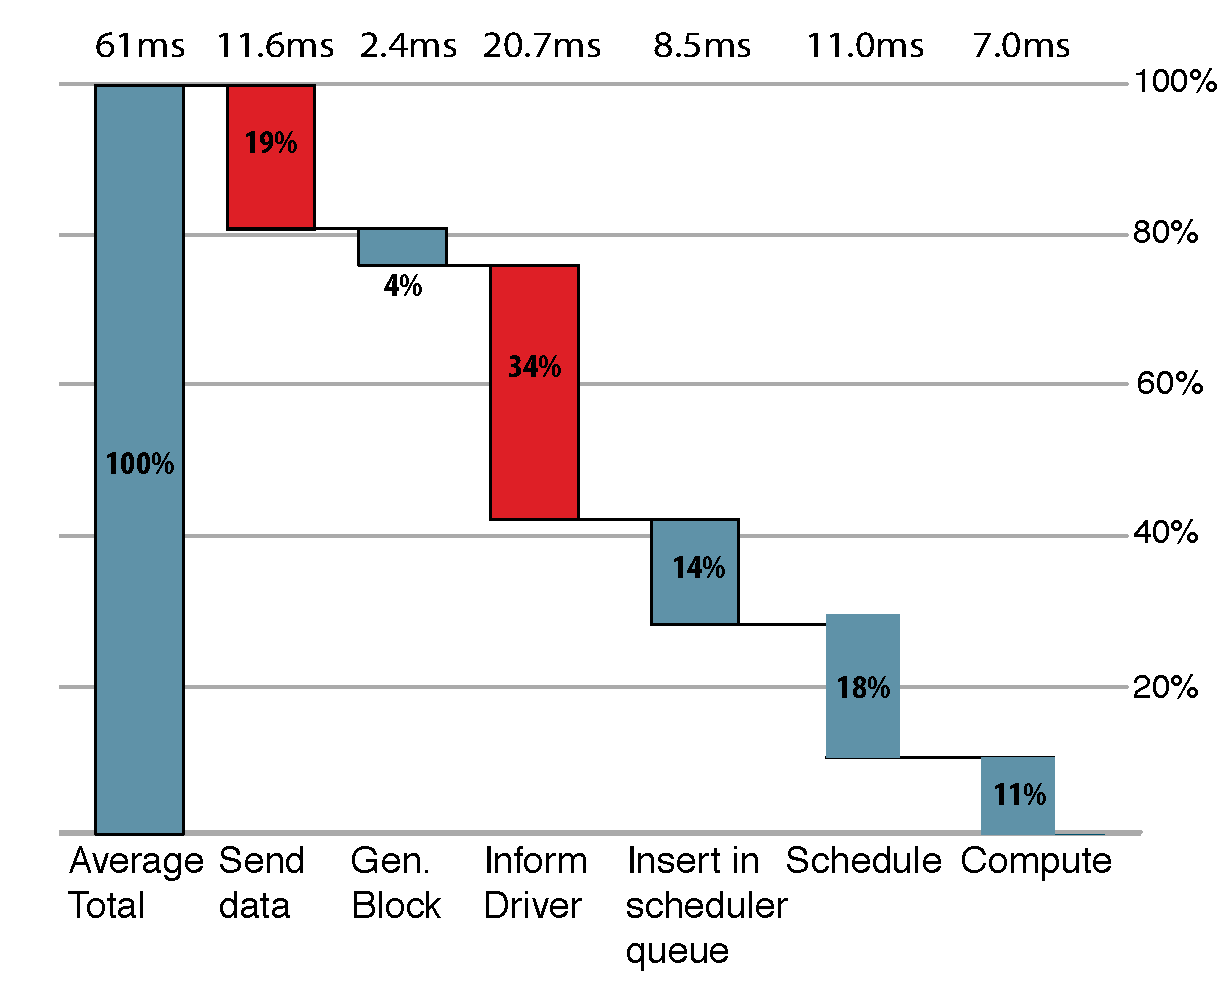
\includegraphics[scale=0.40]{images_graphs/waterfall/Rplots_illustrator.pdf}
  \end{center}
  \caption{}
  \label{fig:SparkStreaming_time_breakdown}
\end{figure}

To better understand the performance and limitations of Spark Streaming we conducted a benchmark study of the system.

To this end we used a synthetic workload to exercise Spark Streaming and measure how the system behaves under different scenarios.
The application consists of a simple transformation of a stream of text records of sizes from 15 to 25 bytes.
In this benchmark we do not focus on the time spent during computation.
This is because first, the computation time is almost always orthogonal to the architecture used.
Secondly, there is other work aimed at improving computation times in streaming or MapReduce systems.
%    There is parallel work on improving the performance of streaming computations that can be used to improve the execution times of tasks.

To run this benchmark, we have deployed a receiver and a record generator in two different machines in the same cluster. 
The record generator generates as many records as necessary to achieve a user-specified throughput.
Each record contains a timestamp that corresponds to the moment of creation of the record as well as a unique ID.
The receiver uses the Spark Streaming API to consume this data. 
A task is generated periodically, according to a user-defined frequency, and scheduled to a node where the data is processed.

We have instrumented the code of Spark Streaming to record the time at which the record transitions a phase (e.g., a task to process a record is scheduled).
%#understand how much time each record stays on each phase of the streaming process.
This allows us to gather 1) the time each record spends on each phase of the streaming process, and 2) the time between the generation of each record and the moment of computation -- end-to-end latency.

%When processing records, the time between the generation of each record and the moment of computation is captured. 
%We refer to this value throughout the paper as the end-to-end latency. 

The results of the first experiment we conducted is captured in Figure~\ref{fig:Batchsize_vs_latency}.
In this graph we show the average end-to-end latency obtained when running Spark Streaming with different batch windows and throughputs. 
Changing the batch window configuration allows us to tune the responsiveness of the system; a lower value means that each records spends less time in memory waiting for a task to be spawned in order to process that same record. 
Varying the number of records generated by the stream source (throughput), allows us to understand how 
Spark behaves when it has to do more/less work per unit of time and how that affects latency.

In the graph we see that for a throughput value of 10Mb/sec Spark.

\begin{figure}[t!]
  \begin{center}
    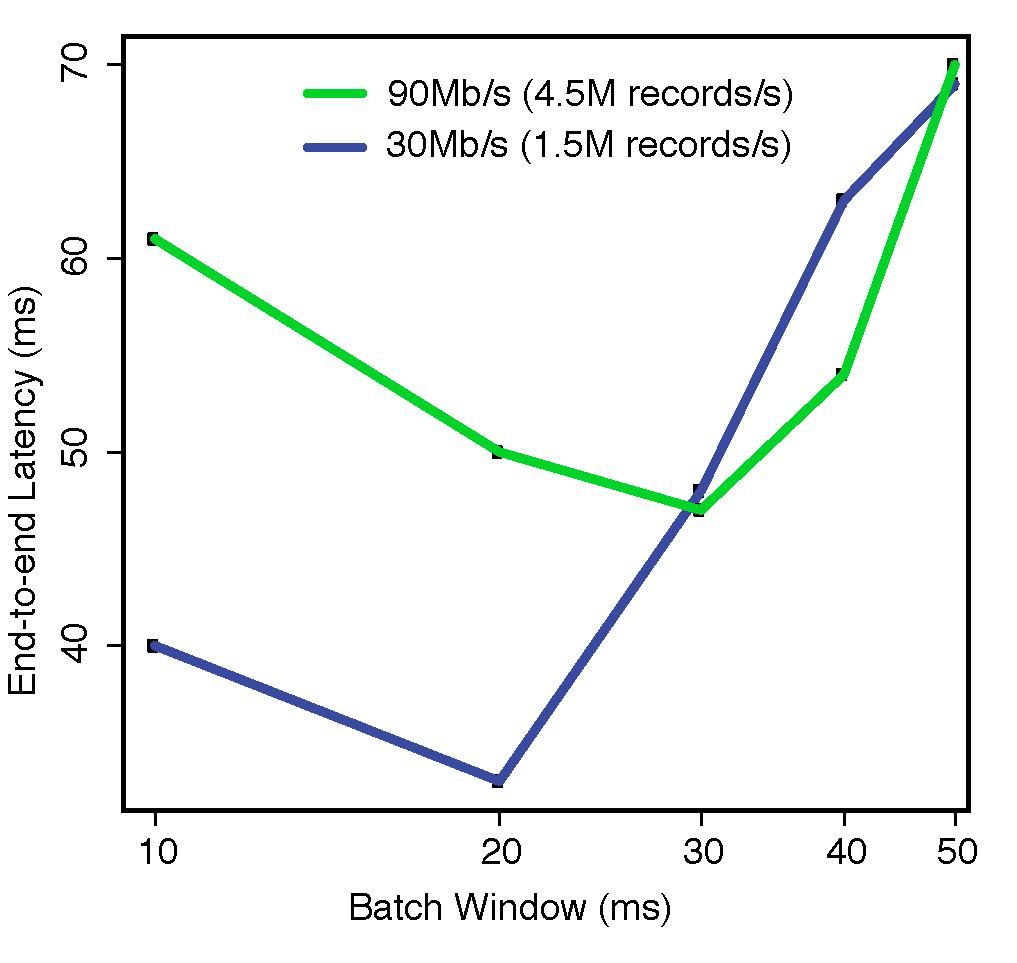
\includegraphics[scale=0.30]{images_graphs/batchsize_vs_latency/batchsize_vs_latency_illustrator.pdf}
  \end{center}
  \caption{}
  \label{fig:Batchsize_vs_latency}
\end{figure}
